\documentclass[tikz,border=6pt]{standalone}
\usepackage[T1]{fontenc}
\usepackage{lmodern}
\usetikzlibrary{arrows.meta,positioning,fit,backgrounds}
\definecolor{hc}{HTML}{2B4FA3}
\definecolor{ac}{HTML}{D7263D}
\definecolor{dc}{HTML}{8A94A0}
\definecolor{ink}{HTML}{1F2933}
\begin{document}
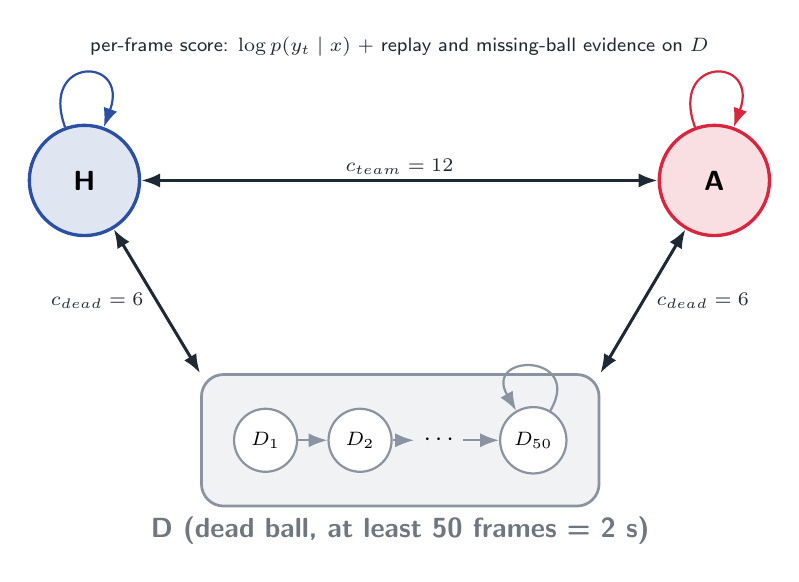
\begin{tikzpicture}[font=\sffamily\small, >={Latex[length=2.4mm]},
  st/.style={circle, draw=#1, fill=#1!15, line width=1.2pt, minimum size=14mm, font=\sffamily\bfseries},
  sub/.style={circle, draw=dc, fill=white, line width=0.8pt, minimum size=8mm, font=\sffamily\scriptsize},
  cost/.style={font=\sffamily\scriptsize, fill=white, inner sep=1.5pt}]
\node[st=hc] (H) at (0,0) {H};
\node[st=ac] (A) at (8,0) {A};
\node[sub] (d1) at (2.3,-3.3) {$D_1$};
\node[sub] (d2) at (3.5,-3.3) {$D_2$};
\node (dots) at (4.5,-3.3) {$\cdots$};
\node[sub] (d50) at (5.7,-3.3) {$D_{50}$};
\begin{scope}[on background layer]
\node[draw=dc, fill=dc!12, rounded corners=8pt, line width=1pt, inner sep=4mm, fit=(d1)(d50),
      label={[font=\sffamily\bfseries, text=dc!80!black]below:D (dead ball, at least 50 frames = 2 s)}] (D) {};
\end{scope}
\draw[->, dc, line width=0.8pt] (d1) -- (d2);
\draw[->, dc, line width=0.8pt] (d2) -- (dots);
\draw[->, dc, line width=0.8pt] (dots) -- (d50);
\draw[->, dc, line width=0.8pt] (d50) to[out=60, in=120, looseness=5] (d50);
\draw[<->, line width=1.1pt, ink] (H) -- node[cost, above] {$c_{team} = 12$} (A);
\draw[<->, line width=1.1pt, ink] (H) -- node[cost, left, xshift=-1mm] {$c_{dead} = 6$} (D.north west);
\draw[<->, line width=1.1pt, ink] (A) -- node[cost, right, xshift=1mm] {$c_{dead} = 6$} (D.north east);
\draw[->, line width=0.8pt, draw=hc] (H) to[out=110, in=70, looseness=5] (H);
\draw[->, line width=0.8pt, draw=ac] (A) to[out=110, in=70, looseness=5] (A);
\node[font=\sffamily\scriptsize, text=ink, align=center] at (4,1.7) {per-frame score: $\log p(y_t \mid x)$ + replay and missing-ball evidence on $D$};
\end{tikzpicture}
\end{document}
